\section{Wireless Sensor Network\\ Testbed Evaluation}
\label{sec-motes}

Having proven our algorithm correct in simple cases and explored the
parameter space using TOSSIM, we then tested RFA on a real sensor
network testbed. The experiments carried out on the 24-node indoor
wireless sensor network testbed, show the performance of our algorithm
running on real hardware, with a complex topology, and experiencing
communication latencies over lossy asymmetric links. The table in
Figure \ref{motelab-summary} summarizes our results, showing that RFA
can rapidly synchronize all the nodes to approx. 100 $\mu$sec.

This section is structured as follows.  First, we describe our testbed
environment, focusing on the significant ways in which the testbed
differs from the TinyOS simulator.  We then describe our use of FTSP
to provide a common global time base for nodes participating in our
experiments. We then discuss our experiments and results, and compare
them to our expectation from theory and simulation.

%% We are currently deploying 30 MicaZ sensor "motes", which consist of
%% an Atmel ATMEGA128L processor running at 7.3MHz, 128KB of read-only
%% program memory, 4KB of RAM, and a Chipcon CC2420 radio operating at
%% 2.4GHz with an indoor range of approximately 100 meters.

\subsection{Testbed Environment}

\begin{figure}
\begin{center}
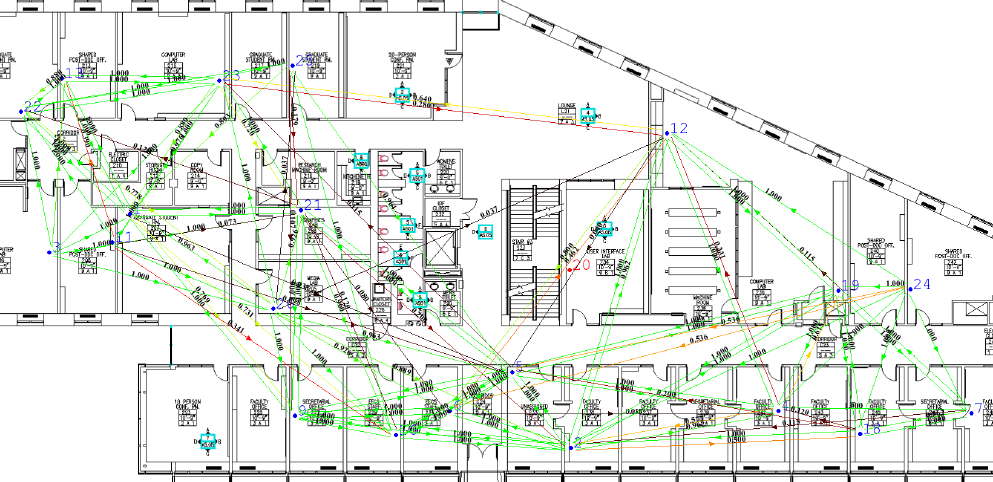
\includegraphics[width=0.85\hsize]{./figures/motelab-map.png}
\end{center}
\caption{Connectivity Map: The distribution and connectivity of sensor
nodes (detailed image at {\tt http://motelab.eecs.harvard.edu/}).}
\label{connectivity-map}
\end{figure}

Our experiments ran on MoteLab~\cite{motelab-spots05-abbrv}, a
wireless sensor network testbed consisting of 24 MicaZ motes
distributed over one floor of our Computer Science and Electrical
Engineering building. The MicaZ motes have a 7.3MHz clock. Each device
is attached to a Crossbow MIB600 interface backchannel board allowing
remote reprogramming and data logging. Messages sent to the nodes'
serial ports are logged by a central server. Using this data-logging
capability, nodes report their firing times as well as information
about firing messages they observe. This information is then used to
evaluate the performance of our algorithm, as well as better
understand its behavior.

\subsubsection{Network Topology}
\label{sec-FTSP}
We conducted our experiments on the most densely populated floor, with
24 nodes. Statistics on message loss rates are calculated periodically
and tend to vary over time. Examining the connectivity map and graph
shown in Figures \ref{connectivity-map} and \ref{connectivity-graph},
one can see that this is a complex multi-hop topology. The layout of
the building produces two cliques of nodes that are connected by high
quality links (less than 20\% message loss) and these cliques are
connected by only a few bridge nodes. Further examination of the
cliques shows that a large fraction of the links are asymmetric in
quality and some nodes (e.g. 2, 26) may have no incoming links of good
quality. This type of complex topology is representative of sensor
networks distributed in a complex environment.



\begin{figure*}[t]
\begin{center}
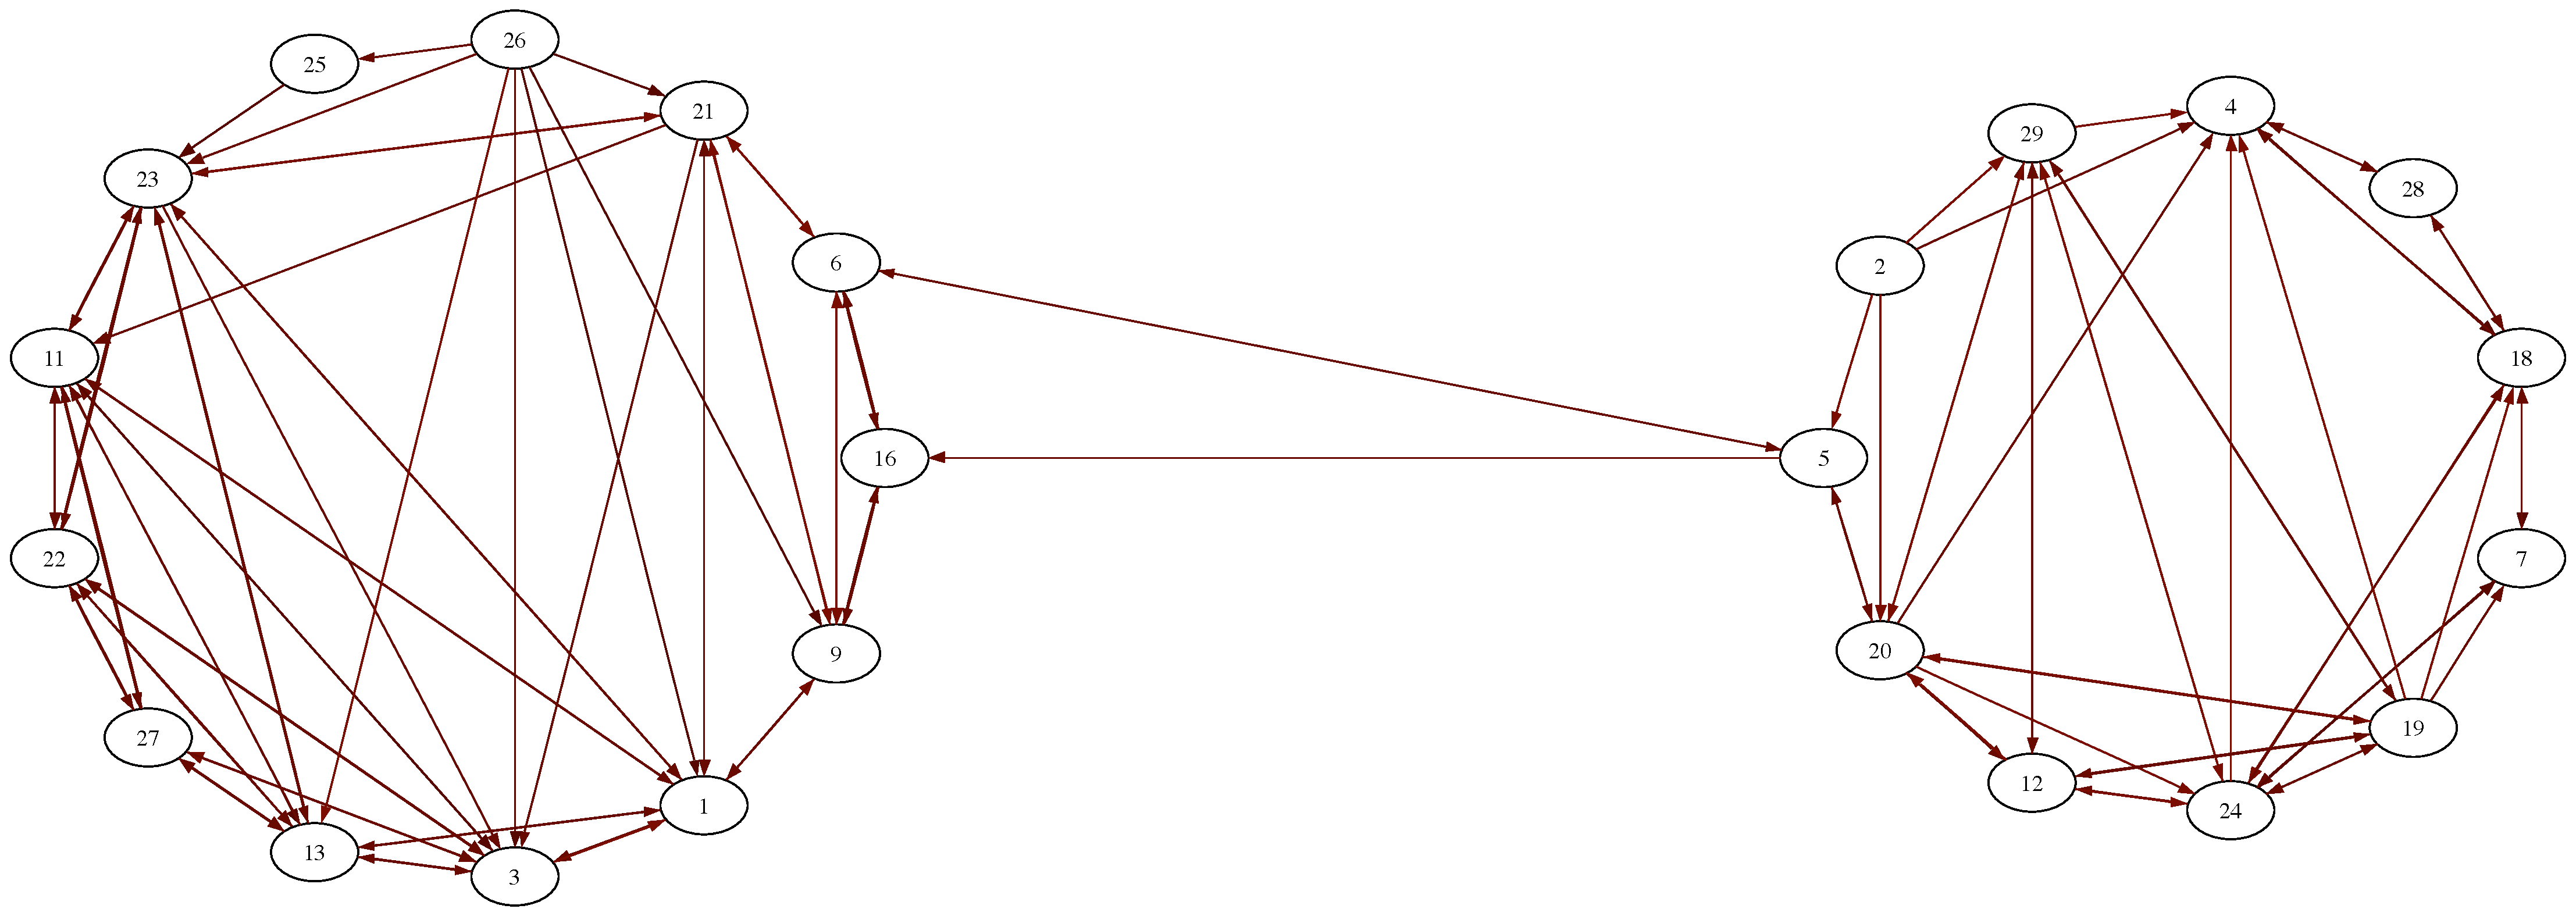
\includegraphics[width=0.8\hsize]{figures/threshold-motelab-0200-e.pdf}
\end{center}
\caption{Connectivity graph of the nodes on our testbed showing links
with better than 80\% packet reception. This reveals two
highly-connected subgraphs and a high percentage of asymmetry in link
quality.}
\label{connectivity-graph}
\end{figure*}




\subsubsection{Time Stamping with FTSP}
\label{FTSP}

In order to evaluate the performance of RFA, we need to time stamp the
firing messages so that we can determine the accuracy with which the
firing phases align. However, this proved to be difficult in our
testbed environment. Unlike TOSSIM, our sensor nodes do not
have access to a global clock. Furthermore, since they are distributed
throughout the building, there is no single base station that can act
as a global observer and provide a common time base \cite{ftsp}. In an
ironic way, evaluating RFA requires an independent and accurate
implementation of time stamping.

%% Once a node is powered up and begins running the only clock it has
%% access to the one driven by its internal oscillator.  The crystal
%% oscillator tolerances of MicaZ and other similar wireless sensor
%% network nodes are on the order of 10 to 100 parts per million.  Over a
%% short period of time these errors prevent nodes from exchanging
%% meaningful timing information using only their local clocks.


To address this difficulty we deployed the Flooding Time
Synchronization Protocol (FTSP)~\cite{ftsp} described in Section
\ref{sec-background}. FTSP provides nodes access to a stable global
clock and allows them to time stamp events with precisions reported in
the tens of microseconds. We characterized the errors in FTSP on our
MoteLab topology in the following way. Nodes log all firing messages
they hear from other nodes and the time stamp that FTSP assigned to
them. For every firing message heard by more than two nodes, we
compute the differences between the times that FTSP reported on each
node, taking the maximum difference between any two stamps. This is
only done for messages where FTSP on both the sender and receiver
reported that the nodes were well-synchronized to the global
clock. The cumulative distribution frequency (CDF) of these errors for
all of our testbed experiments is shown in
Figure~\ref{FTSP-errors}. Note however that the FTSP errors are only
calculated for nodes that are within one hop of each other, therefore we
do not know the error in FTSP between two arbitrary nodes. Given this
caveat, our results show that FTSP can quickly synchronize nodes to
within one hop errors of tens of microseconds.

The use of FTSP as the global clock impacts our experimental results
in two ways. First, our results are pessimistic since their accuracy
is limited by the accuracy of time stamping which is likely to be in
the 5-10 $\mu$sec range. Secondly, this prevents us from making an
objective comparison of accuracy between FTSP and RFA. In the future,
we plan to use more controlled experimental setups to better evaluate
the accuracy of RFA and compare it to other methods.

\begin{figure}
\begin{center}
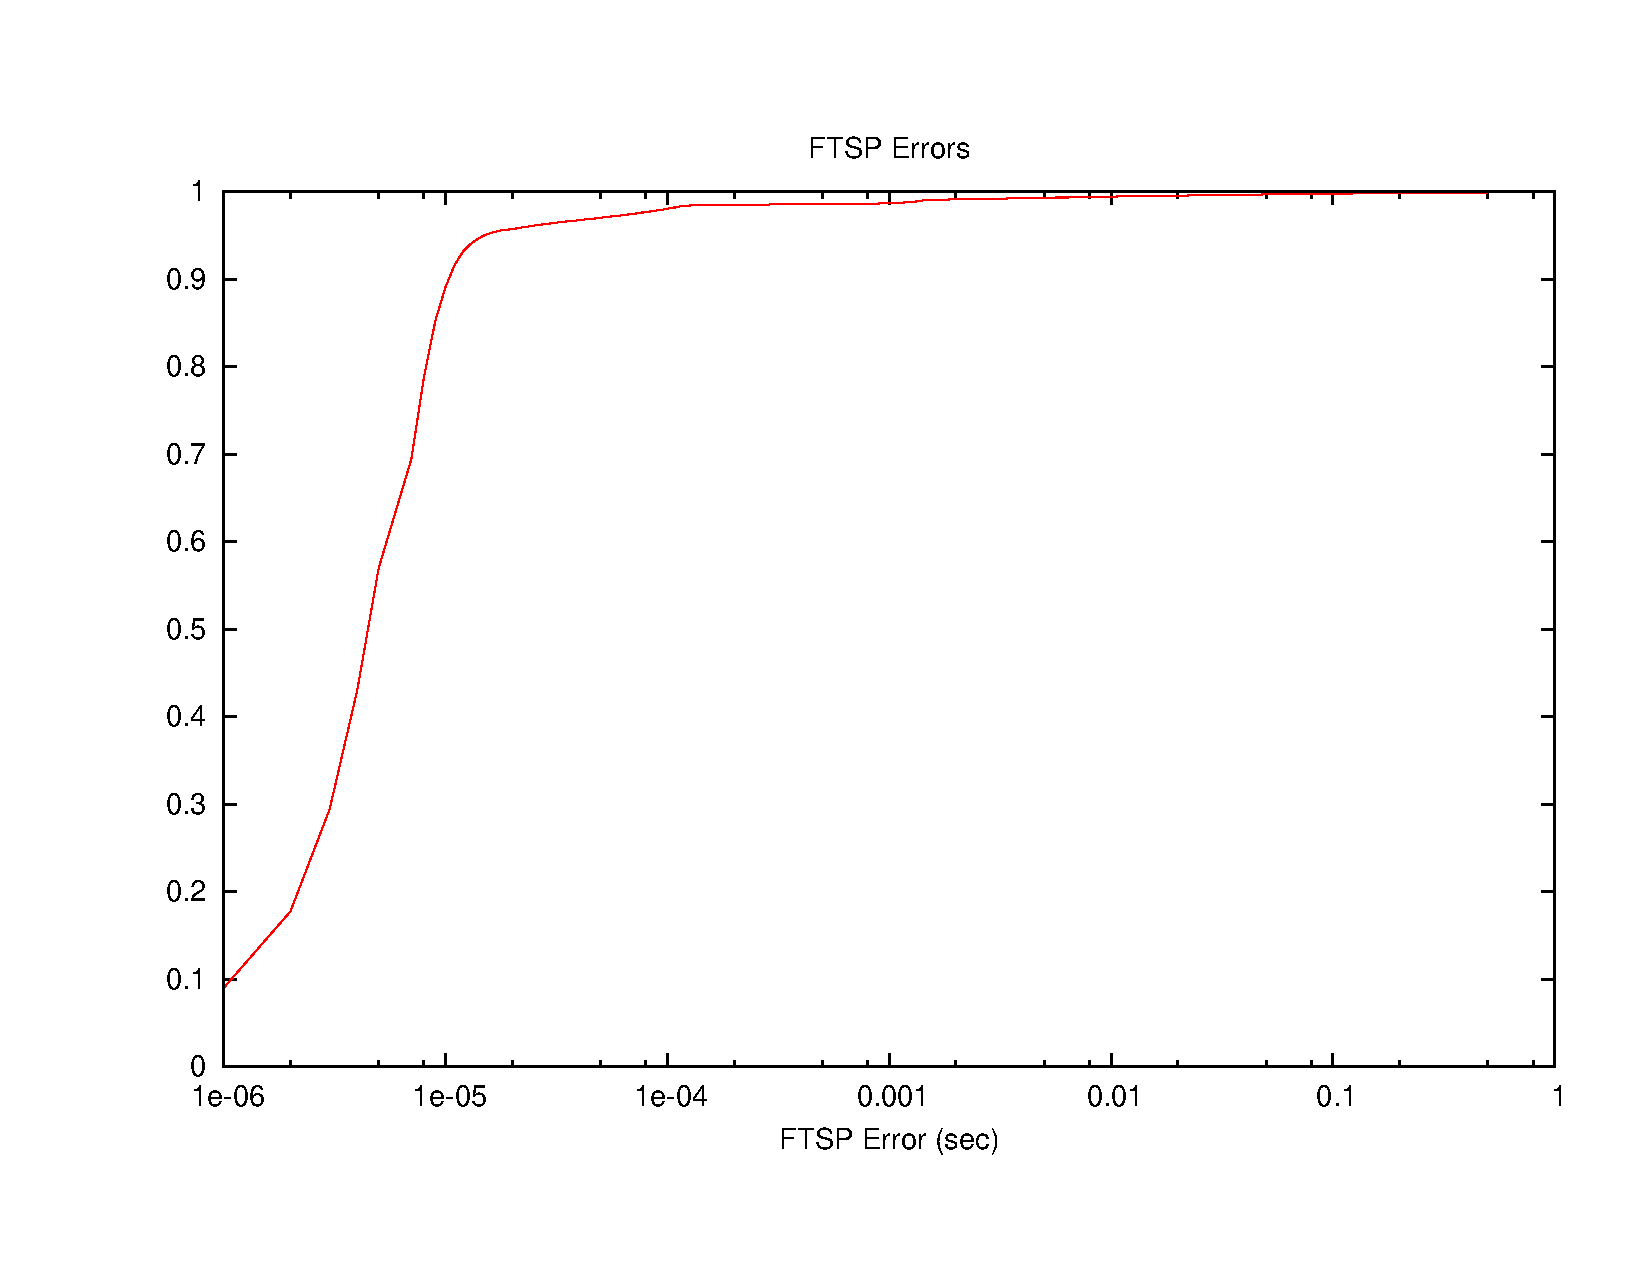
\includegraphics[width=0.8\hsize]{./figures/FTSPERROR.pdf}
\end{center}
\caption {CDF of one hop FTSP error rates collected during all of our
testbed experiments. FTSP provided the global clock for RFA
evaluation.}
\label{FTSP-errors}
\end{figure}


\subsubsection{Differences From the Simulator}
\label{simulator-differences}

Sensor network devices in a real environment exhibit behavior not
modeled by TOSSIM.  Most significant differences for our algorithm are
(1) communication latencies are unpredictable and difficult to measure
accurately, (2) links are asymmetric and fluctuate over time, and (3)
crystal differences cause node clocks to tick at different rates. All
these effects make it difficult for a node to know exactly when
another node fired, and unlikely that it will hear every firing
message sent by its neighbors.

Paradoxically, our testbed is {\em better} than TOSSIM in one very
significant way. The sensor node hardware has a high-precision clock
and high-precision timer components. A TinyOS component written for
our project allows nodes to both locally time stamp and set timers at
$\mu$sec level resolution by multiplexing the {\tt SysTime} and {\tt
MicroTimer} components onto one hardware counter. The simulator TOSSIM
provides 4MHz local time stamping through access to its internal
clock, but no equivalent of the {\tt MicroTimer} component, forcing us
to rely on the standard TinyOS {\tt Timer} component with its
millisecond resolution. This limits the resolution of the jumps a node
can take and therefore the algorithm achieves only millisecond
accuracy in simulation. As we were using the simulator primarily to
explore the impact of parameter and topology, we felt the lack of
precision this introduced was acceptable.  The higher frequency {\tt
MicroTimer} component is the primary reason that group spread results
from our testbed experiments are much better than the simulation,
which at first would seem surprising.

\subsection{Performance Evaluation} 

\label{performance-evaluation}


The table in Figure \ref{motelab-summary} summarizes the results from
our experiments. We conducted four experiments with firing function
constants (FFC) 100, 250, 500 1000.

In each of these experiments the network achieves synchronicity. In
the case with a FFC of 100, the network is synchronized within 5
minutes, with a group spread of 131 $\mu$sec. As expected from our
theoretical and simulation studies, the time to synchronize increases
with larger firing function constants. The table also shows the 50th
and 90th percentile group spread, and Figure \ref{groupspread-cdf}
plots the group spread CDFs for each of the four FFCs. As we can see
they are striking similar, aligning with our expectations from theory
and simulations that group spread does not depend on the FFC value.

These results are very encouraging, given the caveats on our time
stamping and the complexity of the testbed environment. However, there
are also several features which are still unexplained and we plan to
investigate these more in the future. Here we discuss two examples.

One observation from the CDF plot in Figure \ref{groupspread-cdf} is
that there seems to be a limit on the achievable group spread of
around 100 $\mu$sec.  This could be related to FTSP accuracy, but it
is also affected by clock skew. We expect clock skew to impact the
accuracy of RFA because the M\&S model upon which it is based assumes
that nodes agree on a fixed firing period. However, two perfectly
synchronized nodes will diverge on the very next firing by the amount
of drift that exists in their clocks --- introducing an error that is on
the order of the crystal accuracy. This causes the nodes to constantly
readjust their phases. Clock skew also impacts the accuracy indirectly
when nodes use the message delay (measured by the sender's clock) to
adjust their own phase. In the future we plan to investigate the
effects of clock skew more rigorously and look at alternate models of
synchronization, such as synchronized clapping, where both frequency
and phase are adjusted.

%% note clock skew is 1-100 parts per million, for a ~8MHz clock this is
%% at most 100/8 ~ 10usec

\begin{figure}[t]
\begin{center}
\begin{small}
\begin{tabular}{|lllll|} \hline
{\em FFC constant} & 
{\em Time to} & 
{\em 50th pct} &
{\em 90th pct} &
{\em Mean group} \\
{\em } &
{\em sync (sec)} &
{\em spread} & 
{\em spread} & 
{\em std dev} \\
&
&
{\em ($\mu$sec)} & 
{\em ($\mu$sec)} & 
\\
\hline
100 & 284.3 & 131.0 & 4664.0 & 410.4 \\
250 & 343.6 & 128.0 & 3605.0 & 572.2 \\
500 & 678.1 & 154.0 & 30236.0 & 1327.8 \\
1000 & 1164.4 & 132.0 & 193.0 & 63.6 \\
\hline
\end{tabular}
\end{small}
\end{center}
\caption{Summary of Testbed Results. Four experiments were run on the
24 node testbed, with different firing function constants (where $FFC
= 1/\epsilon$) As expected, the time to synchronize increases with
FFC. The 50th percentile group spread is similar for all four
experiments.}
\label{motelab-summary}
\end{figure}

\begin{figure}
\begin{center}
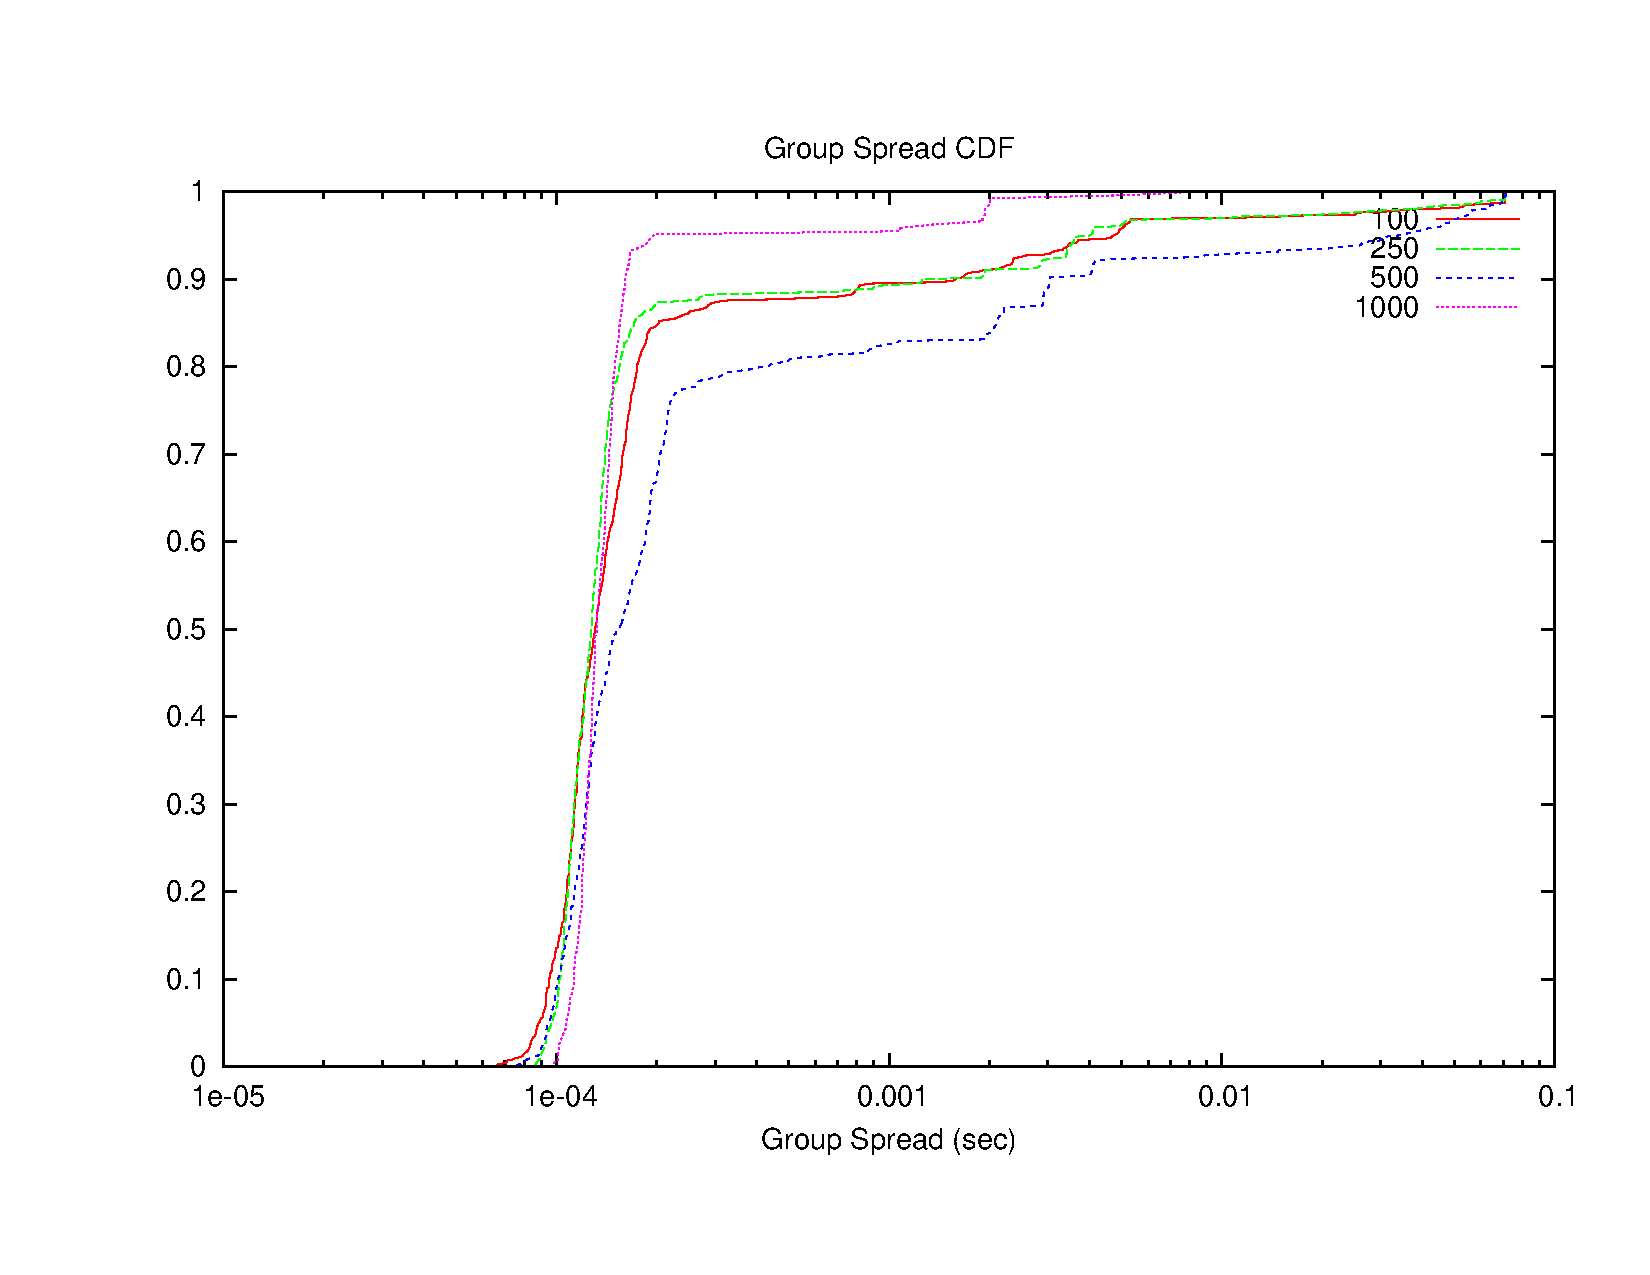
\includegraphics[width=0.8\hsize]{./figures/CDFTOT.pdf} 
\end{center} 
\caption{CDF of RFA Group Spread. The four different firing function
constants in the testbed experiments produce similar levels of
synchronicity.}
\label{groupspread-cdf} 
\end{figure} 

%% This was completely bogus! and caught by the reviewers.
%% the theory and simulation suggest the OPPOSITE!
%% \caption{CDF of RFA Group Spread: The four different firing function
%% constants in the testbed experiments produce remarkably similar levels
%% of synchronicity. Our simulator and theoretical results indicate that the
%% tightness achieved should scale with the firing function constant chose, and
%% so these results are somewhat confusing.  However, we do achieve good
%% synchronicity across all four firing function constants.


A second observation arises from looking at the group spread over
time. We observed that even after tight groups form, occasionally
disturbances still occur during the experiment. We refer to these as
{\em dispersive events}. Figure \ref{phaseplot-motelab-specific} (a)
shows an example of a dispersive event where the nodes fall out of
phase and the system recovers from this impulse over the next few
firing periods. Figure \ref{phaseplot-motelab-specific} (b) shows a
different time course with the occurrence of two dispersive events
which cause the group to spread over approximately 0.1 $sec$
range. Note that these dispersive events are included in the data in
Table ~\ref{motelab-summary} and impact the 90th percentile group
spread. Analysis of the information collected during this experiment
showed no clear reason for this spurious firing. It is unlikely to be
caused by the algorithm, since the extent of dispersion is larger than
the maximum jump possible given the FFC. What is encouraging is that
the recovery from the 100 msec range dispersive events takes only a
few rounds to achieve, thus showing that the system can recover
quickly from perturbation. However, a more rigorous instrumentation
and experimentation setup will be required to pinpoint the causes
behind this behavior.

\begin{figure*}[t]
\begin{center}
(a)
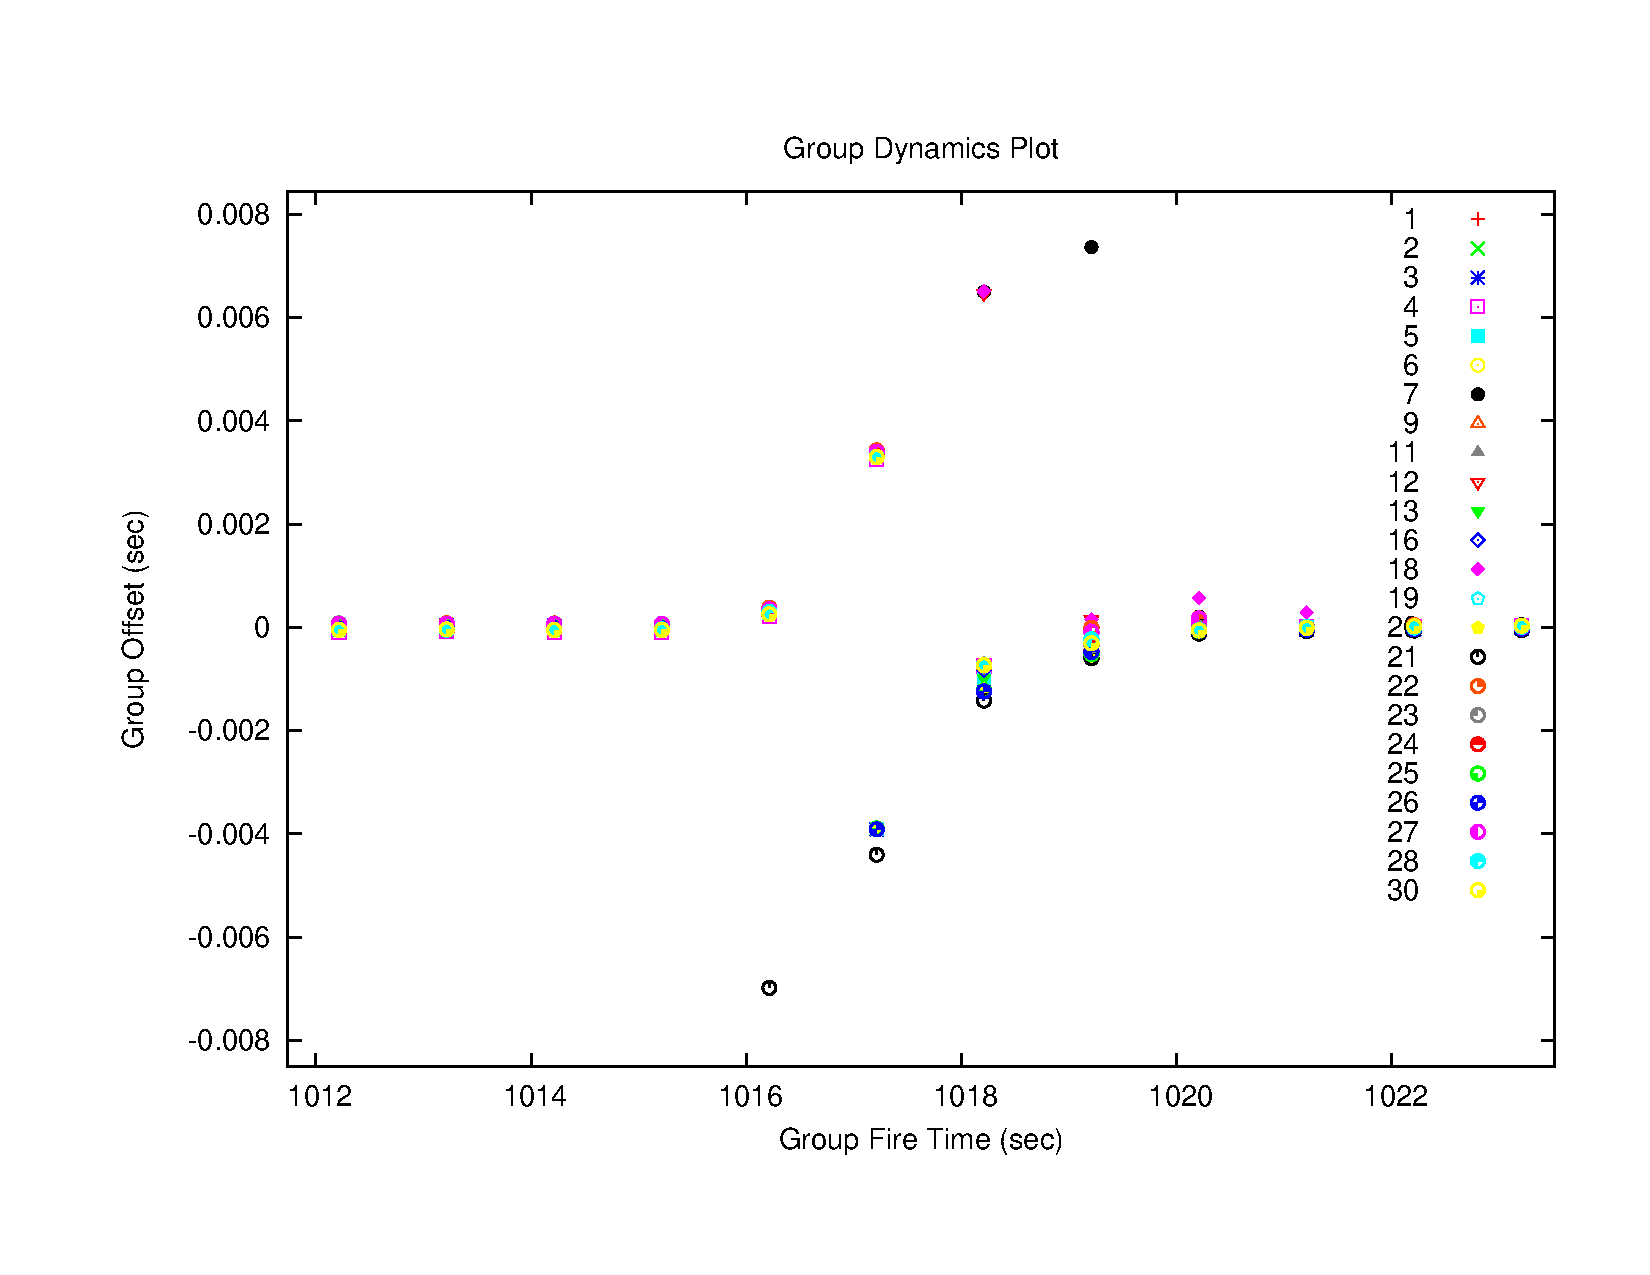
\includegraphics[width=0.4\hsize]{./figures/GROUPDYNAMICS-SPECIFIC.pdf}
(b)
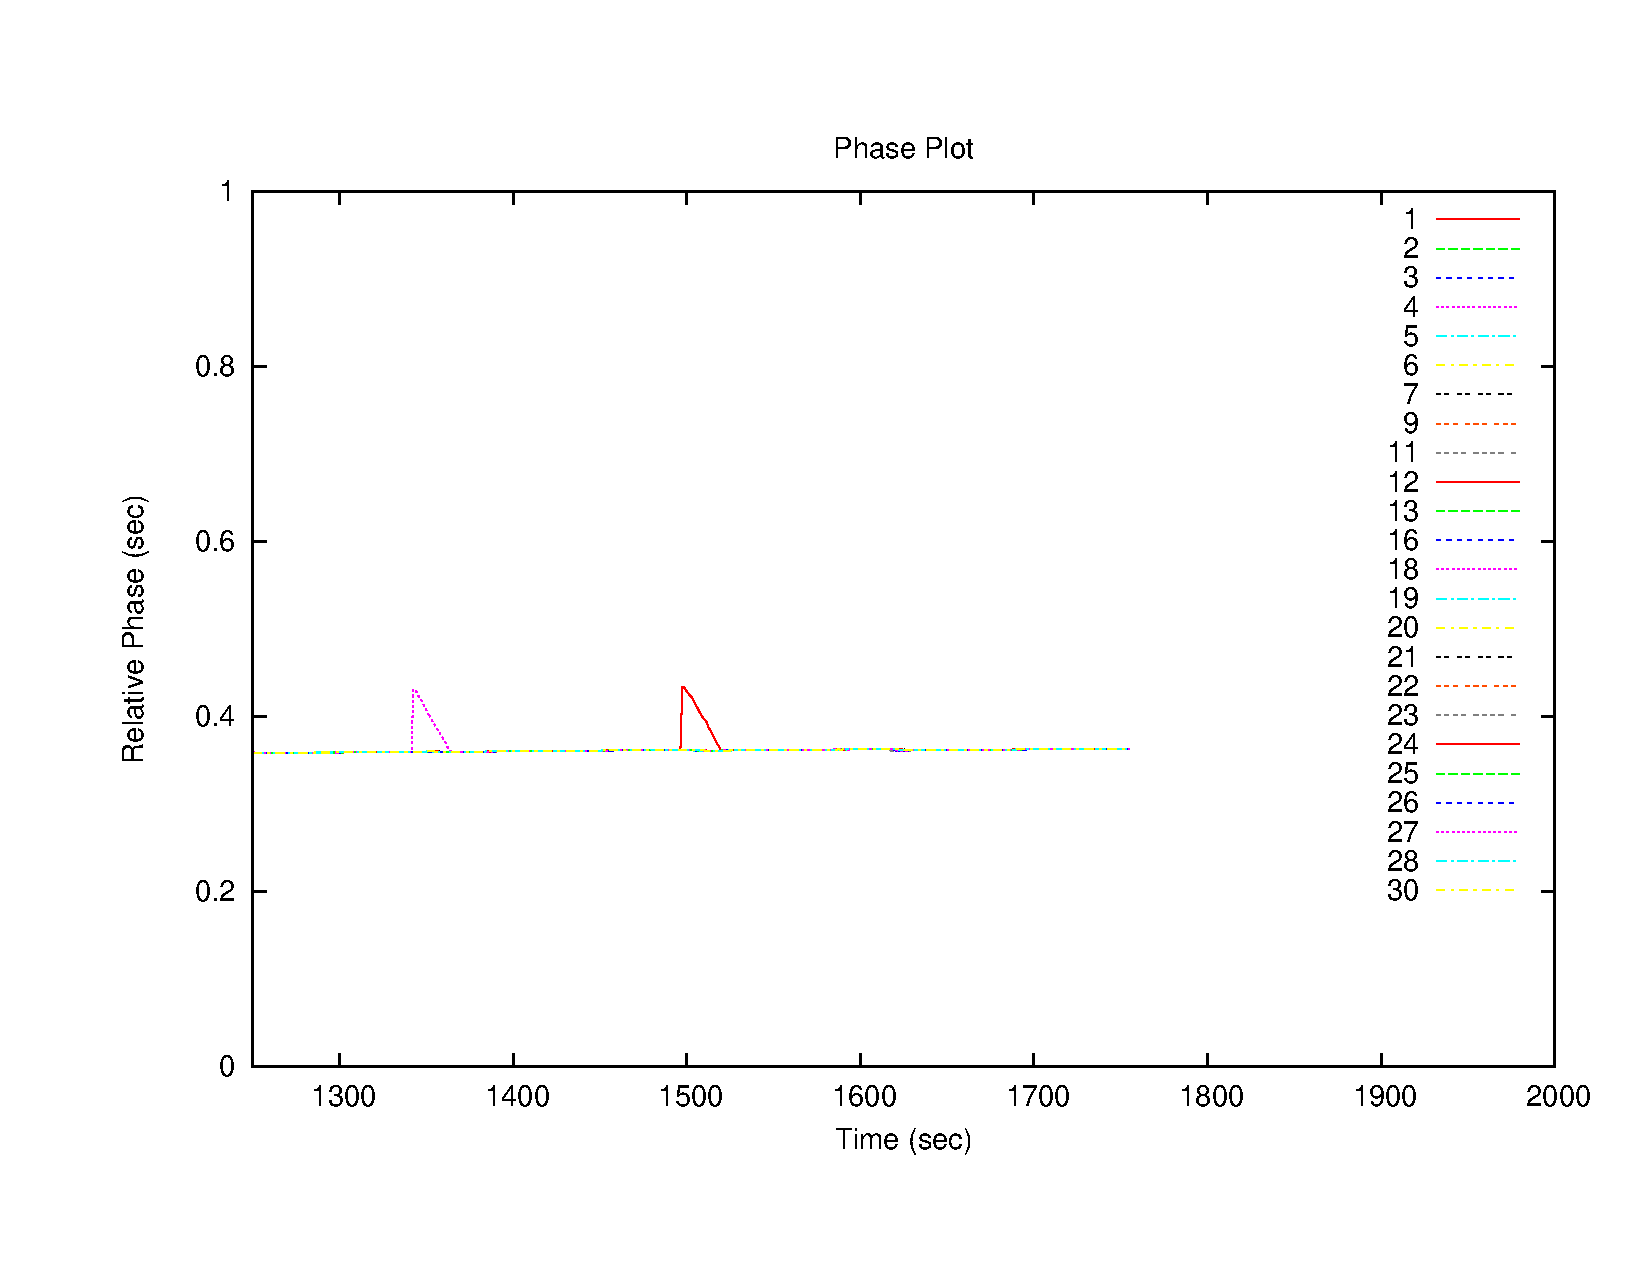
\includegraphics[width=0.4\hsize]{./figures/PHASEPLOT-SPECIFIC.pdf}
\end{center}
\caption{Dispersive events (a) This plot shows the group dynamics for
several firing periods following the effect of one node falling out of
sync. Nodes offsets against the average group firing time are plotted
with respect to time. (b) This plot shows a different example, with
FFC=1000. After the system has stabilized there are still two cases
where nodes jump out of phase and are re-incorporated into the group.}
\label{phaseplot-motelab-specific}
\end{figure*}


%% RAD
%%
%% I removed these because it is not clear to me the either of these
%% are potential explanations for the dispersive events. One should
%% be able to validate/substantiate these ideas by looking at the actual data.
%% the long-lost nbrs doesn't make sense since all of the nodes are tightly
%% clustered so even if you heard a long lost neighbor, the correction could never
%% be that large. Unless th message delay time was garbled....

%% what puzzles me the most is that the dispersion is huge, maybe even too large
%% given the FFC which limits the amount of corrective action possible in one
%% step - so it seems more as if the nodes somehow took a big hiccup somewhere
%% Given the our experinec with the counter roll-over problems like in simulation
%% seems premature to spend this much time discussing possible issues

%% Actually, to substantiate my argument
%% In the figure X, with FFC=1000
%% a dispersive event is approximate 0.1 sec in height.
%% With the FFC constant, a node could move only .001sec at most in one cycle.
%%

%%%%%%
%% \begin{itemize}
%% \item {\bf Clock Skew:} The error associated between any two clocks
%% acts as a constant dispersive force limiting the accuracy of our
%% algorithm.  Based on their interactions, all nodes may attempt to
%% choose a next firing time that is perfectly aligned. Because of clock
%% skew they will end up distributed with a spread dependent on the
%% accuracy of the crystals used to drive their hardware counters.

%% Clock skew also impacts the timing of radio events.  The delay to send a
%% message is measured by the sender and applied by the receiver.  Differences
%% between node clocks will cause an error when the receiver applies this delay
%% to calculate when the sender fired in its local time frame.

%% \item {\bf Long-lost Neighbors:} Lossy links can cause a node to suddenly
%% hear from another node that it has not heard from for a long time, again
%% precipitating a large correction.
%% \end{itemize}


%% RAD I took out this graph since it was adding much to the text or 
%% the other two dispersive event pictures which are much more informative
%% \begin{figure}[p]
%% \begin{center}
%% 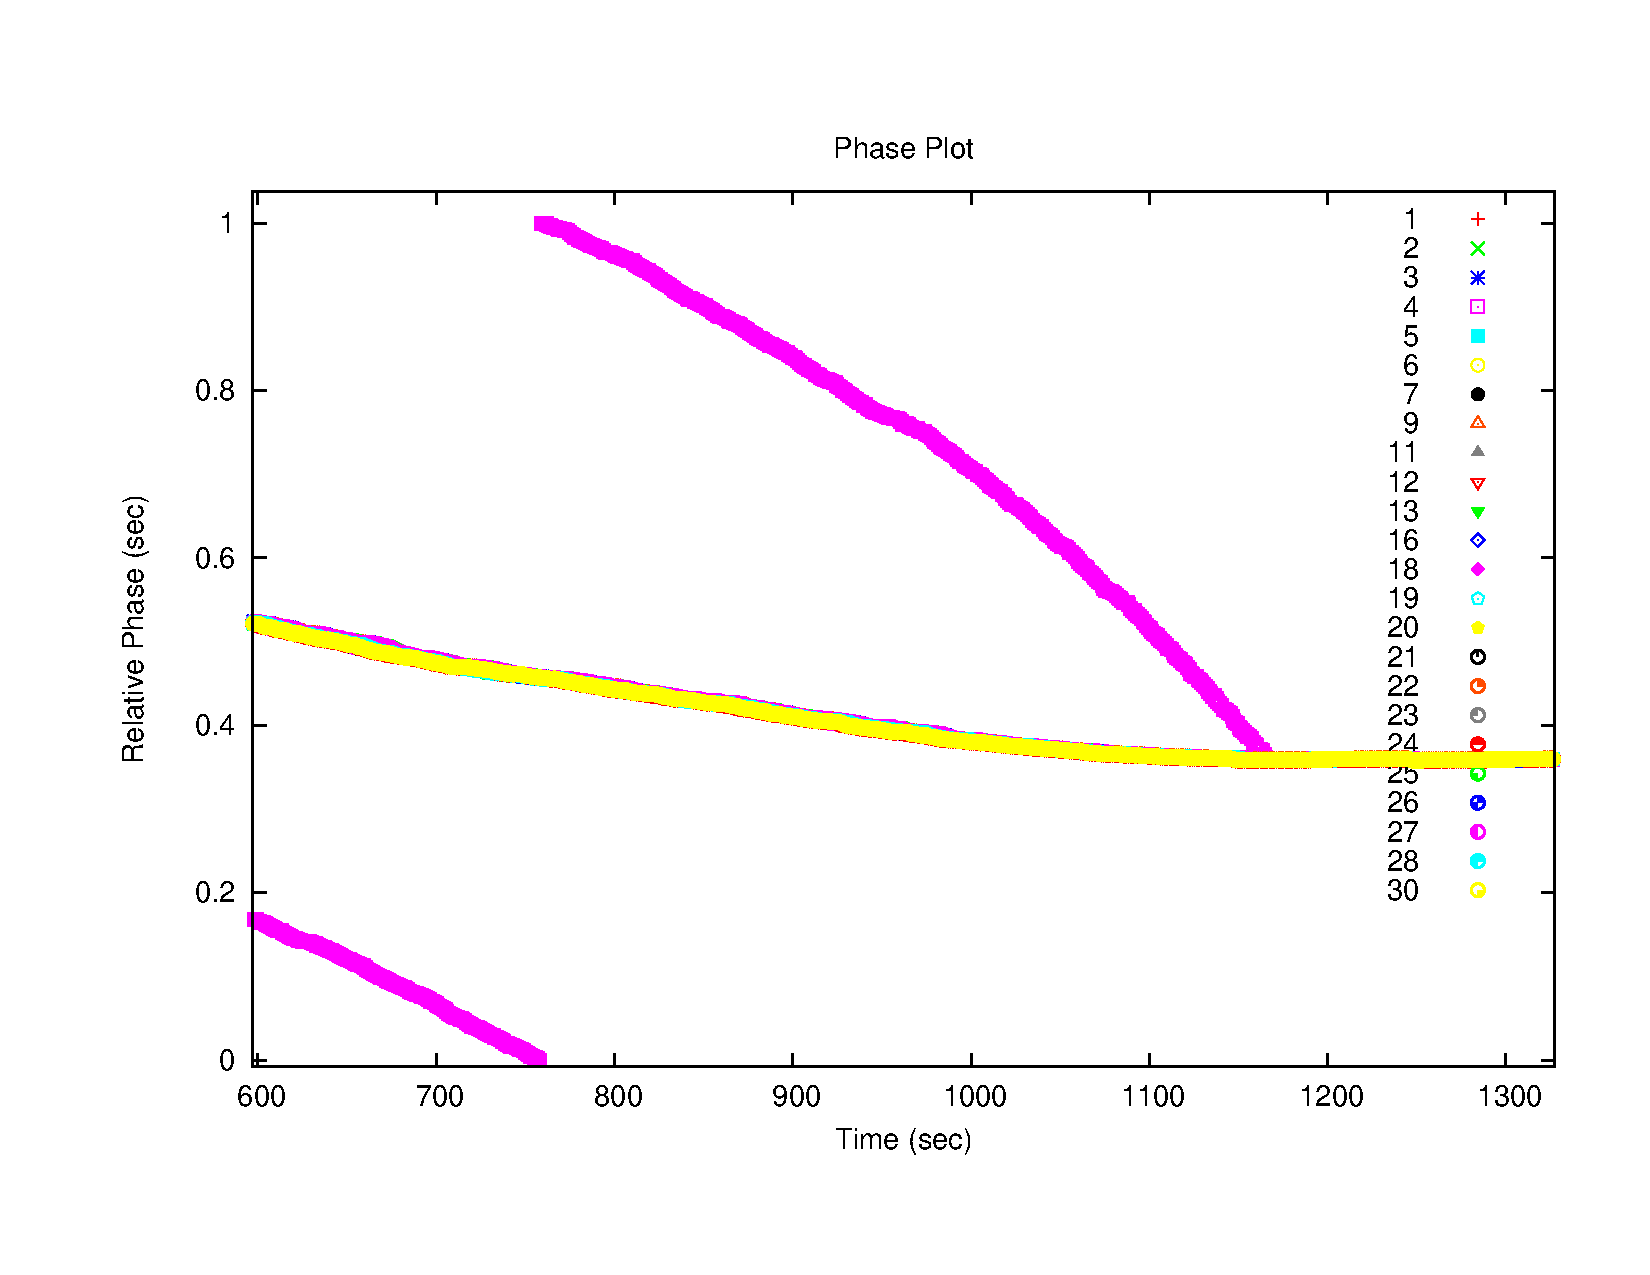
\includegraphics[width=0.8\hsize]{./figures/PHASEPLOT.pdf}
%% \end{center}
%% \caption {\small {\bf Phase Portrait for 1000 Firing Function Constant.}
%% {\em
%% This plot shows a phase portrait for a testbed experiment with a firing
%% function constant of 1000 exhibiting a striking display of node capture.
%% Node 18 is the last node to join the group and the phase portrait shows it
%% racing around to catch the existing group.  As it draws closer the period of
%% the larger group relaxes as it is less and less influenced by the outlier. 
%% }}
%% \label{phaseplot-motelab}
%% \end{figure}

